\documentclass{article}

\usepackage{graphicx}
\usepackage{tikz}
\usepackage{tikzsymbols}
\usetikzlibrary{calc,patterns,shapes.geometric}
\pagestyle{empty}
\usepackage[margin=0pt]{geometry}
\geometry{papersize={14in,12in}}

\def\centerarc[#1](#2)(#3:#4:#5){\draw[#1] ($(#2)+({#5*cos(#3)},{#5*sin(#3)})$) arc (#3:#4:#5);}

\begin{document}
	\begin{figure}
		\centering
		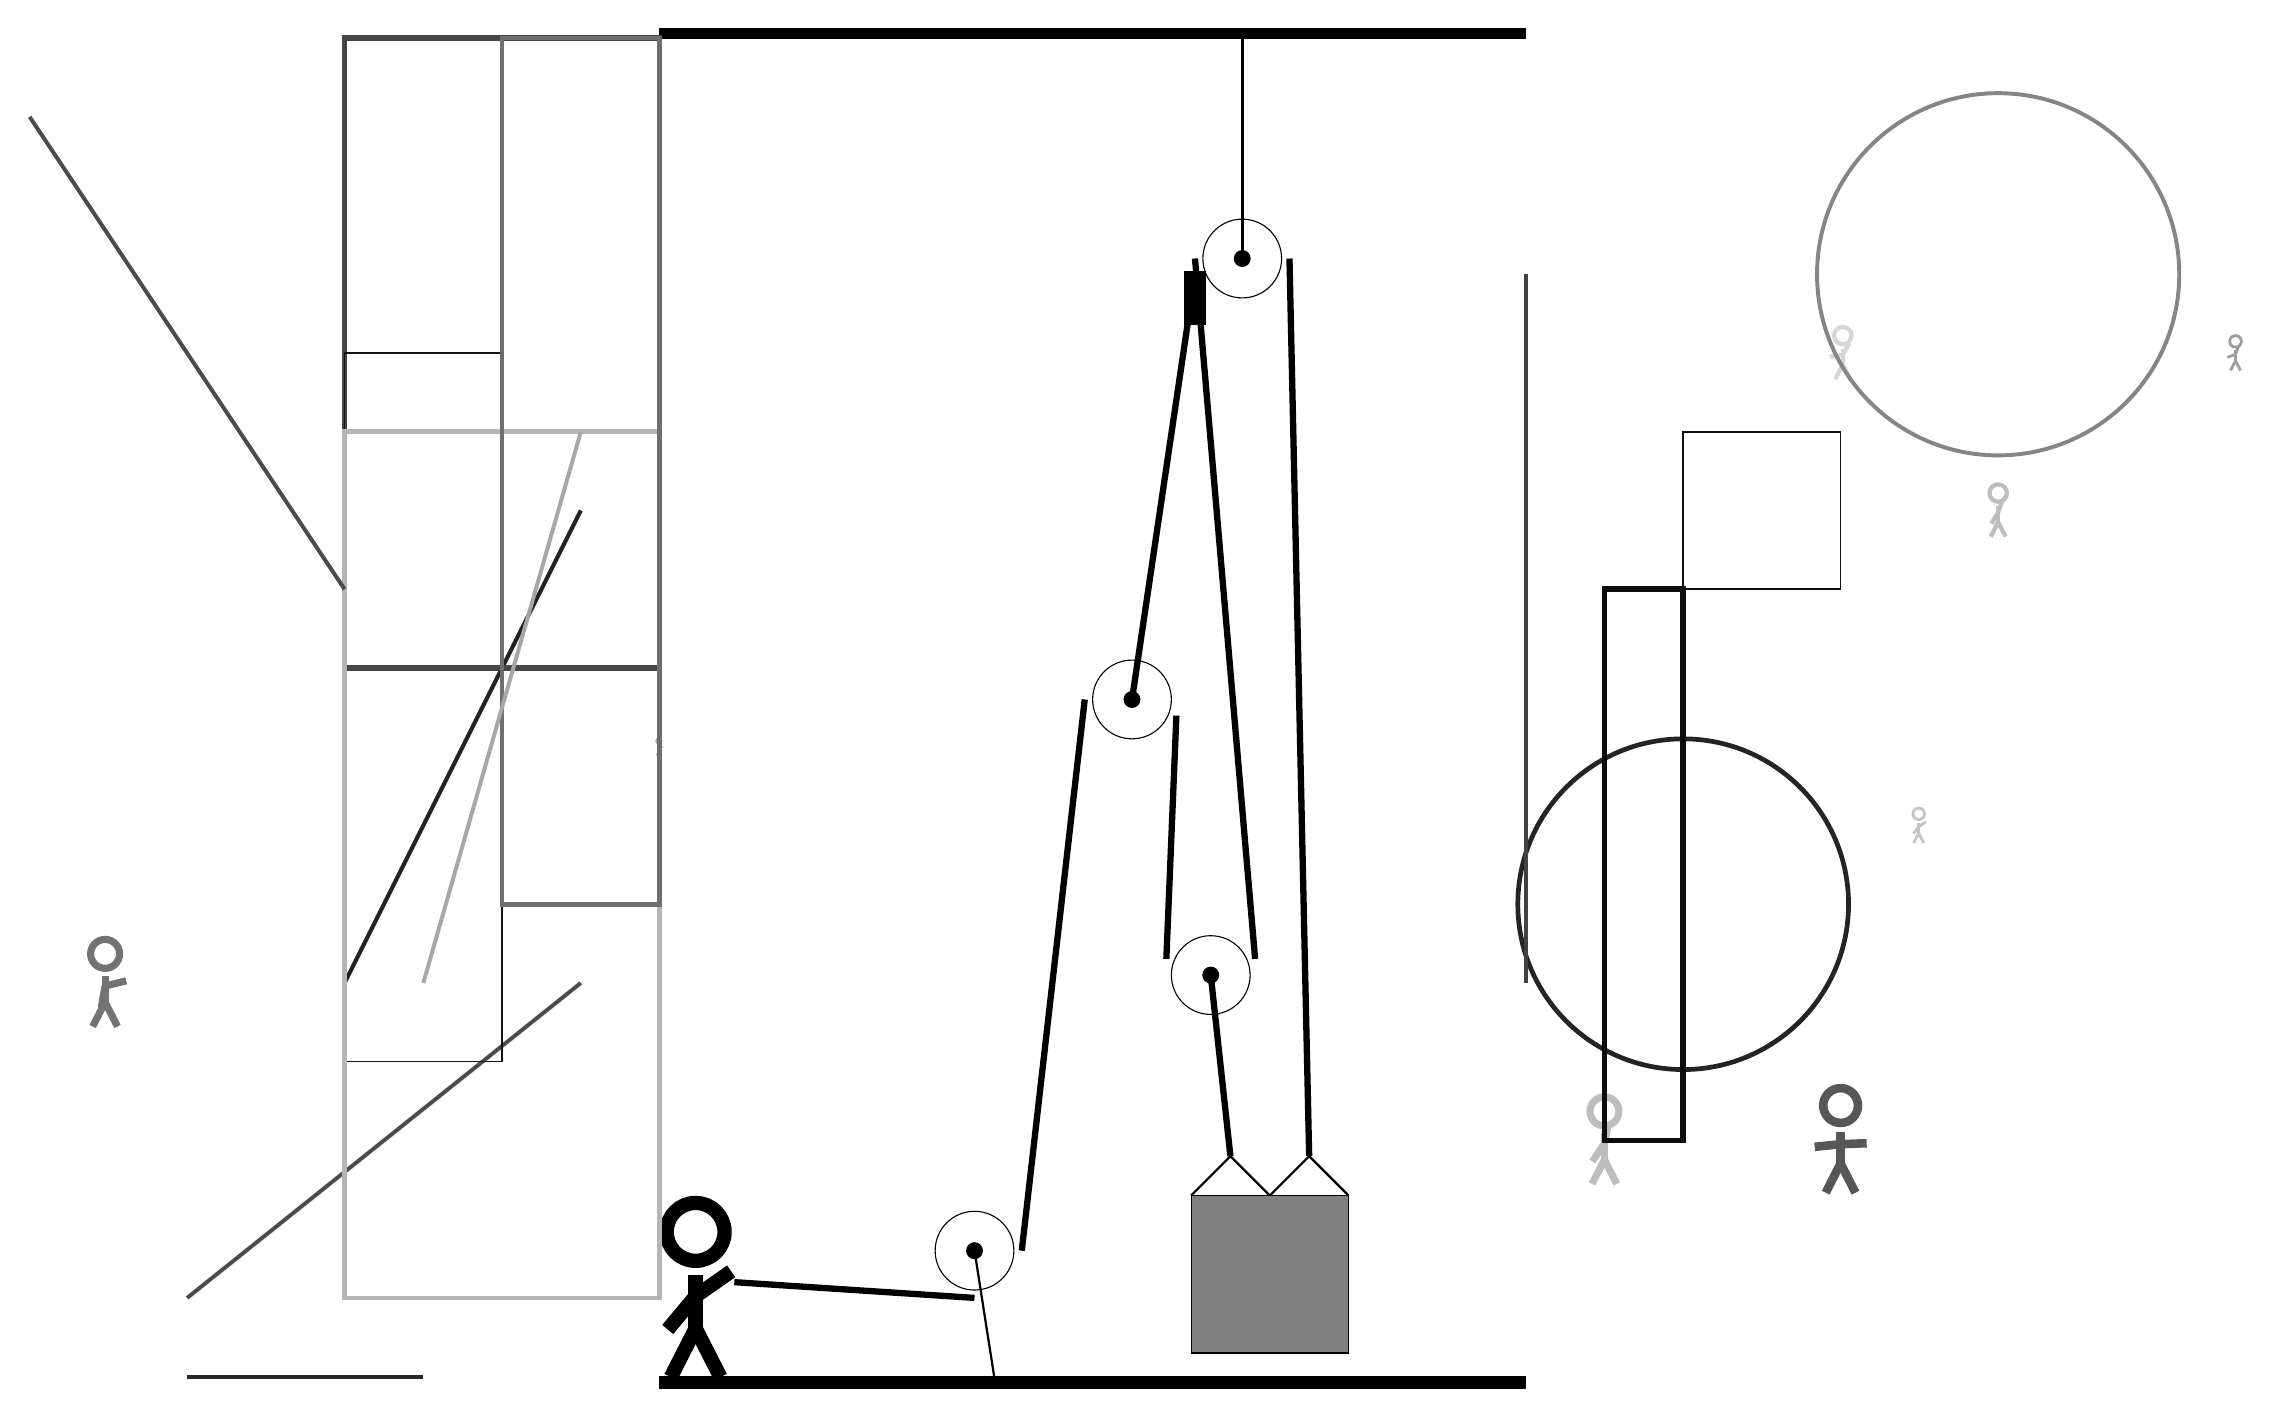
\begin{tikzpicture}
			%%%%% START %%%%%
			
			\draw[fill=black] (-6, 14) rectangle (5, 14.125);
			
			\draw (0, 5.6) circle (0.5);
			\draw[fill=black] (0, 5.6) circle (0.1);
			
			\draw (1, 2.1) circle (0.5);
			\draw[fill=black] (1, 2.1) circle (0.1);
			
			\draw (1.4, 11.2) circle (0.5);
			\draw[fill=black] (1.4, 11.2) circle (0.1);
			\draw[very thick] (1.4, 11.2) -- (1.4, 14);
			
			\draw (-2, -1.4) circle (0.5);
			\draw[fill=black] (-2, -1.4) circle (0.1);
			\draw[thick] (-2, -1.4) -- (-1.75, -3);
			
			
			\draw[thick]  (0.75, -0.7) -- (1.25, -0.2) -- (1.75, -0.7) -- (2.25, -0.2) -- (2.75, -0.7);
			\draw[fill=black!50] (0.75, -0.7) rectangle (2.75, -2.7);
			\draw[line width=0.8mm] (-5.05, -1.8) -- (-2, -2.0);
			\centerarc[line width=0.8mm](-2, -1.4)(270:360:0.6);
			\draw[line width=0.8mm] (-1.4, -1.4) -- (-0.6, 5.6);
			\draw[line width=0.8mm] (0, 5.6) -- (0.8, 11.0);
			\draw[line width=0.8mm, fill=black](0.7, 10.4) rectangle (0.9, 11.0);
			\centerarc[line width=0.8mm](0, 5.6)(-20:180:0.6);
			\draw[line width=0.8mm] (0.5638, 5.3948) -- (0.4362, 2.3052);
			\centerarc[line width=0.8mm](1, 2.1)(160:380:0.6);
			\draw[line width=0.8mm] (1.5638, 2.3052) -- (0.8, 11.2);
			\draw[line width=0.8mm](1, 2.1) -- (1.25, -0.2);
			\centerarc[line width=0.8mm](1.4, 11.2)(0:180:0.6);
			\draw[line width=0.8mm] (2.0, 11.2) -- (2.25, -0.2);
			
			\node at (-5.5, -1.9) {\Strichmaxerl[10][50][35]};
			
			\draw[line width=0.5mm, color=black!87](-7, 8) -- (-10, 2);
			
			\draw[line width=0.5mm, color=black!70](-7, 2) -- (-12, -2);
			\node[line width=0.3mm, color=black!55] at (-13, 2) {\Strichmaxerl[5][80][14]};
			\draw[line width=0.7mm, color=black!73] (-6, 14) rectangle (-10, 6);
			
			\node[line width=0.2mm, color=black!26] at (6, 0) {\Strichmaxerl[5][56][79]};
			\draw[line width=0.2mm, color=black!92] (-8, 1) rectangle (-10, 10);
			\draw[line width=0.6mm, color=black!29] (-6, -2) rectangle (-10, 9);
			\draw[line width=0.2mm, color=black!94] (7, 7) rectangle (9, 9);
			\node[line width=0.3mm, color=black!16] at (9, 10) {\Strichmaxerl[3][8][61]};
			
			\draw [line width=0.6mm, color=black!86](7, 3) circle (2.1);
			\draw[line width=0.5mm, color=black!27] (-7, 4) rectangle (-7, 4);
			\node[line width=0.7mm, color=black!66] at (9, 0) {\Strichmaxerl[6][6][2]};
			\draw[line width=0.5mm, color=black!85](-9, -3) -- (-12, -3);
			
			\draw[line width=0.5mm, color=black!74](5, 2) -- (5, 11);
			\node[line width=0.2mm, color=black!26] at (11, 8) {\Strichmaxerl[3][59][70]};
			\node[line width=0.4mm, color=black!33] at (-6, 5) {\Strichmaxerl[1][89][5]};
			
			\draw[line width=0.7mm, color=black!95] (6, 0) rectangle (7, 7);
			\node[line width=0.2mm, color=black!23] at (10, 4) {\Strichmaxerl[2][52][35]};
			\draw [line width=0.5mm, color=black!48](11, 11) circle (2.3);
			\node[line width=0.6mm, color=black!38] at (14, 10) {\Strichmaxerl[2][21][70]};
			\draw[line width=0.5mm, color=black!70](-10, 7) -- (-14, 13);
			
			\draw[line width=0.6mm, color=black!57] (-8, 3) rectangle (-6, 14);
			\draw[line width=0.5mm, color=black!35](-9, 2) -- (-7, 9);
			
			\draw[fill=black] (-6, -3) rectangle (5, -3.15);
			
			%%%%% END %%%%%
		\end{tikzpicture}
	\end{figure}	
\end{document}